% 这个版本的 CVPR 模板由 Ming-Ming Cheng 提供。
% 如果您发现了错误,请留下问题:
% https://github.com/MCG-NKU/CVPR_Template。

%\documentclass[review]{cvpr}
\documentclass[final]{cvpr}
\usepackage[UTF8]{ctex}
\usepackage{enumitem}
\usepackage{times}
\usepackage{epsfig}
\usepackage{graphicx}
\usepackage{amsmath}
\usepackage{amssymb}
\usepackage{makecell}
\usepackage{booktabs}
\usepackage[table,xcdraw]{xcolor}
\usepackage{multirow}
\usepackage{bbm}


% 在 hyperref 之前包含其他包。

% 如果您注释掉 hyperref 然后取消注释它,您应该删除
% egpaper.aux 然后重新运行 latex。 (或者只需在第一次 latex
% 运行时按 'q',让它完成,您应该就可以了)。
\usepackage[pagebackref=true,breaklinks=true,colorlinks,bookmarks=false]{hyperref}

\def\cvprPaperID{4107} % *** 在此处输入 CVPR 论文 ID
\def\confYear{CVPR 2021}
%\setcounter{page}{4321} % 仅用于最终版本


\begin{document}

\title{铁路不是火车:显著性作为伪像素监督 \ 用于弱监督语义分割}

\author{Seungho Lee\thanks{ 表示同等贡献。}\\
延世大学\\
{\tt\small seungholee@yonsei.ac.kr}
% 对于所有作者都在同一机构的论文,
% 省略以下行直到关闭“}”。
% 可以使用“\and”添加其他作者和地址,
% 就像第二个作者一样。
% 为了节省空间,请使用电子邮件地址或主页,而不是两者
\and
Minhyun Lee\footnotemark[1]\\
延世大学\\
{\tt\small lmh315@yonsei.ac.kr}
\and 
Jongwuk Lee\\
成均馆大学\\
{\tt\small jongwuklee@skku.edu}
\and 
Hyunjung Shim\thanks{Hyunjung Shim 是通讯作者。}\\
延世大学\\
{\tt\small kateshim@yonsei.ac.kr}
}

\maketitle
\thispagestyle{empty}
\pagestyle{empty}

%%%%%%%%% 摘要

\begin{abstract}
现有使用图像级弱监督的弱监督语义分割(WSSS)研究存在几个局限性:稀疏的对象覆盖、不准确的对象边界以及来自非目标对象的共现像素。为了克服这些挑战,我们提出了一种新颖的框架,即显式伪像素监督(EPS),通过结合两种弱监督从像素级反馈中学习;图像级标签通过定位图提供对象身份,而来自现成显著性检测模型的显著性图提供丰富的边界。我们设计了一种联合训练策略,以充分利用两种信息之间的互补关系。我们的方法可以获得准确的对象边界并丢弃共现像素,从而显著提高伪掩码的质量。实验结果表明,所提出的方法通过解决 WSSS 的关键挑战显著优于现有方法,并在 PASCAL VOC 2012 和 MS COCO 2014 数据集上实现了新的最先进性能。代码可在 \href{https://github.com/halbielee/EPS}{https://github.com/halbielee/EPS} 获取。
\end{abstract}


\section{介绍}

弱监督语义分割(WSSS)利用弱监督(例如,图像级标签~\cite{pathak2015constrained, pinheiro2015image}、涂鸦~\cite{lin2016scribblesup} 或边界框~\cite{khoreva2017simple})并旨在实现与需要像素级标签的全监督模型相竞争的性能。大多数现有研究采用图像级标签作为分割模型的弱监督。WSSS 的整体流程包括两个阶段。首先,使用图像分类器为目标对象生成伪掩码。然后,使用伪掩码作为监督训练分割模型。生成伪掩码的流行技术是类激活映射(CAM)~\cite{zhou2016learning},它提供与其图像级标签对应的对象定位图。由于全监督(即像素级注释)和弱监督(即图像级标签)语义分割之间的监督差距,WSSS 面临以下关键挑战:1)定位图仅捕获目标对象的一小部分~\cite{zhou2016learning},2)它遭受对象边界不匹配的困扰~\cite{kim2017two},以及 3)它几乎无法将共现像素与目标对象分开(例如,火车上的铁路)~\cite{kolesnikov2016seed}。

\begin{figure}[t]
\centering
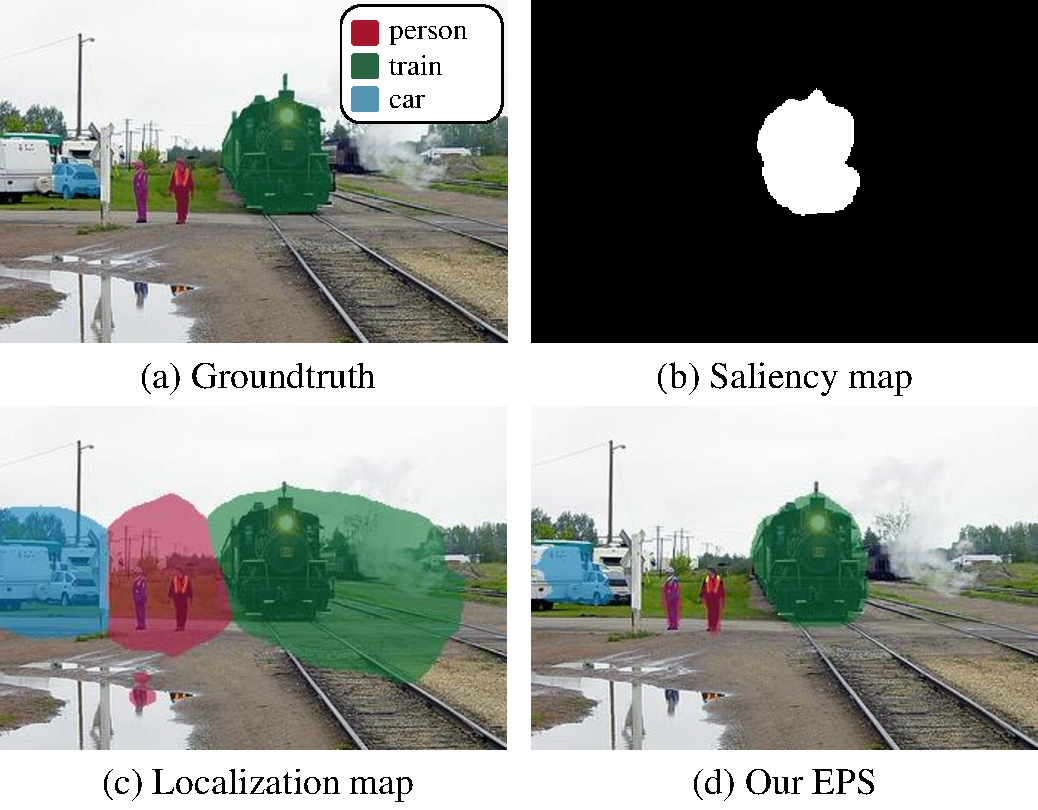
\includegraphics[width=8 cm]{figures/fig_concept.pdf}
\caption{Motivating example of utilizing both the saliency map and the localization map for WSSS. (a) Groundtruth, (b) saliency map via PFAN~\cite{zhao2019pyramid}, (c) localization map via CAM~\cite{zhou2016learning} and (d) our EPS utilizing both the saliency map and the localization map for training a classifier. Note that the saliency map cannot capture \emph{person} and \emph{car} while our result can correctly restore them, and the localization map overly captures two objects.} \vspace{-2mm}
\label{fig:concept}
\end{figure}

为了解决这些问题,现有的研究可以分为三个支柱。第一种方法通过擦除像素~\cite{choe2020attention,kim2017two, li2018tell}、集成得分图~\cite{jiang2019integral, lee2019ficklenet}或使用自监督信号~\cite{wang2020self}来扩展对象覆盖范围以捕捉对象的全部范围。然而,由于没有线索来指导对象的形状,它们无法确定目标对象的准确边界。第二种方法专注于改进伪掩码的对象边界~\cite{fan2020learning,chen2020boundary}。由于它们有效地学习了对象边界,因此它们自然地将伪掩码扩展到边界。然而,它们仍然无法区分非目标对象与目标对象的重合像素。这是因为前景和背景之间的强相关性(即,共现)几乎无法与归纳偏差(即,观察目标对象及其重合像素的频率)区分开来,如~\cite{choe2020evaluating}所示。最后,第三种方法旨在通过使用额外的真实掩码~\cite{BMVC2016_92}或显著性图~\cite{oh2017exploiting, yao2020saliency}来缓解共现问题。然而,\cite{BMVC2016_92,li2018tell}需要强像素级注释,这与弱监督学习范式相去甚远。\cite{oh2017exploiting}对显著性图的错误很敏感。此外,\cite{yao2020saliency}未能覆盖对象的全部范围,并且存在边界不匹配的问题。

在本文中,我们的目标是通过充分利用定位图(即,使用图像级标签训练的图像分类器的CAM)和显著性图(即,现成的显著性检测模型的输出~\cite{hou2017deeply,nguyen2019deepusps,zhao2019pyramid})来克服WSSS的三个挑战。我们专注于定位图和显著性图之间的互补关系。如图~\ref{fig:concept}所示,定位图可以区分不同的对象,但不能有效地分离它们的边界。相反,虽然显著性图提供了丰富的边界信息,但它并未揭示对象的身份。从这个意义上说,我们认为使用这两种互补信息的方法可以解决WSSS的性能瓶颈。

为此,我们提出了一种新的WSSS框架,称为\emph{显式伪像素监督(EPS)}。为了充分利用显著性图(即,前景和背景),我们设计了一个分类器来预测$C+1$类,包括$C$个目标类和背景类。我们利用$C$个定位图和背景定位图来估计显著性图。然后,显著性损失被定义为显著性图和我们估计的显著性图之间的像素级差异。通过引入显著性损失,模型可以通过所有类的伪像素反馈进行监督。我们还使用多标签分类损失来预测图像级标签。因此,我们训练分类器以优化显著性损失和多标签分类损失,协同优化背景和前景像素的预测——我们发现我们的策略可以改进显著性图(第~\ref{section3.3}节和图~\ref{fig:sal})和伪掩码(第~\ref{section:5.1}节和图~\ref{fig:ablation})。

我们强调,由于显著性损失通过伪像素反馈惩罚边界不匹配,它可以强制我们的方法学习对象的准确边界。作为副产品,我们还可以通过将地图扩展到边界来捕捉整个对象。因为显著性损失有助于将前景(例如,火车)与背景分开,我们的方法可以将共现像素(例如,铁路)分配给背景类。实验结果表明,我们的EPS在PASCAL VOC 2012和MS COCO 2014数据集上取得了显著的分割性能,记录了新的最先进的准确性。

\section{相关工作}

\noindent\textbf{弱监督语义分割。}
WSSS 的一般流程是从分类网络生成伪掩码,并使用伪掩码作为监督来训练分割网络。由于图像级标签中边界信息的稀缺,许多现有方法存在伪掩码不准确的问题。为了解决这个问题,交叉图像亲和性~\cite{fan2020cian}、知识图谱~\cite{liu2020leveraging} 和对比优化~\cite{sun2020mining, zhang2020splitting} 被用来提高伪掩码的质量。\cite{chang2020weakly} 提出了一种自监督任务来发现子类别,以强制分类器改进 CAM。\cite{ahn2019weakly, ahn2018learning} 通过计算像素之间的亲和性隐式利用边界信息。\cite{zhang2020reliability} 专注于生成可靠的像素级注释,并设计了一个端到端网络来生成分割图。\cite{huang2018weakly, kolesnikov2016seed} 通过利用边界损失来训练分割网络。最近,\cite{araslanov2020single} 使用了一个基于单一分割的模型,并采用自监督训练方案。\cite{fan2020employing} 通过利用多个不完整的伪掩码来关注分割网络的鲁棒性。

\begin{figure*}[t]
\centering
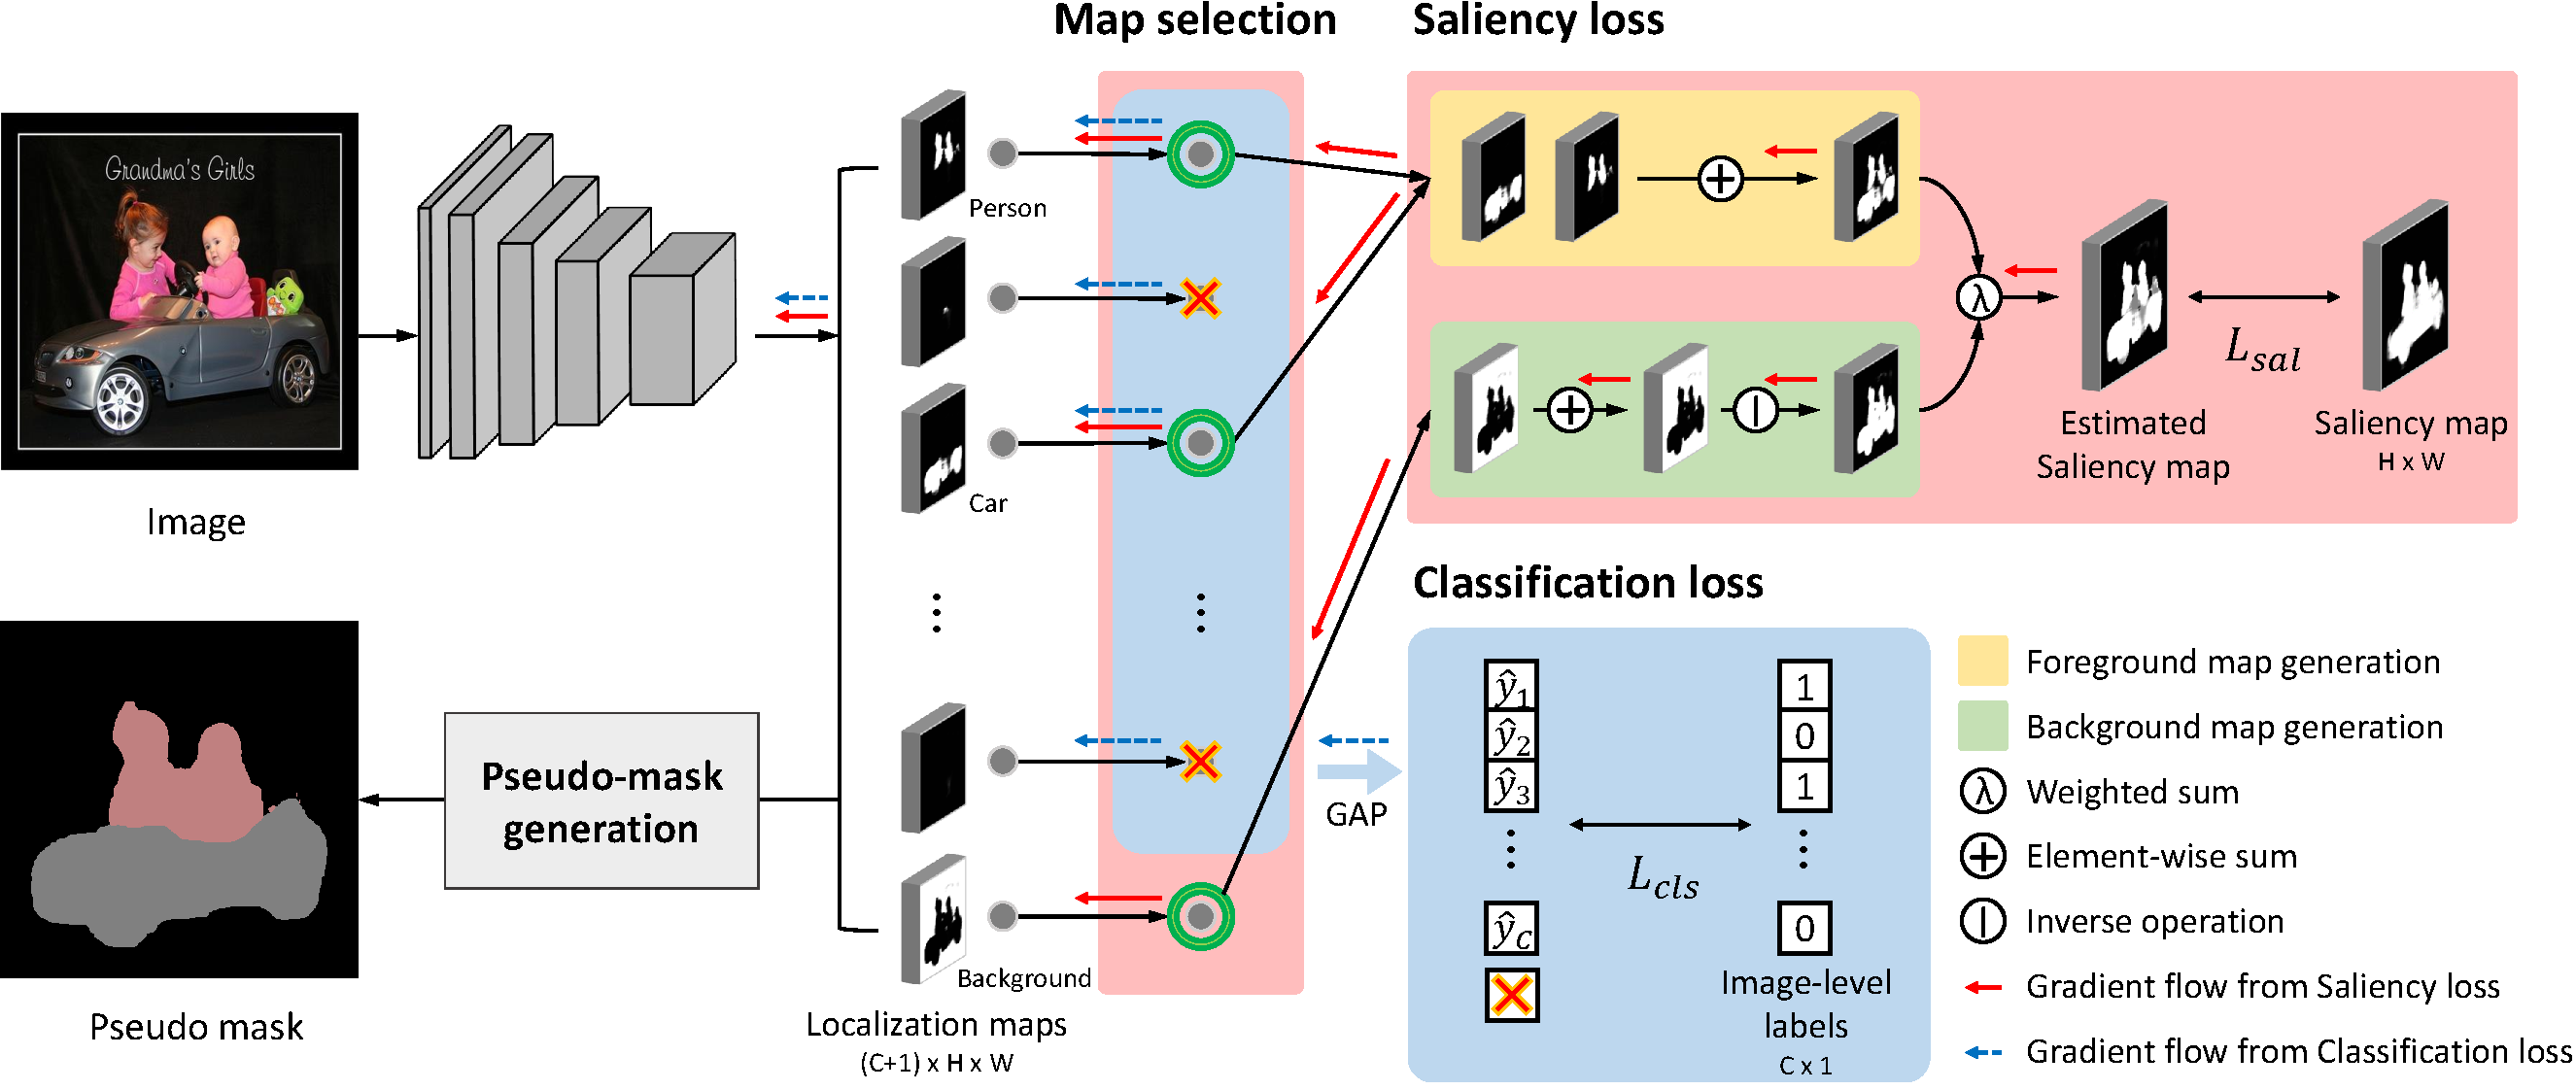
\includegraphics[width=16cm]{figures/framework.pdf}
\caption{我々のEPSの全体的なフレームワーク。$C+1$のローカライゼーションマップがバックボーンネットワークから生成されます。実際の顕著性マップは、既製の顕著性検出モデルから生成されます。ターゲットラベルのためのいくつかのローカライゼーションマップは、推定顕著性マップを生成するために選択的に使用されます(セクション~\ref{section3.2})。全体的なフレームワークは、顕著性損失と分類損失と共に共同で訓練されます(セクション~\ref{section3.3})。} \vspace{-2mm}
\label{fig:framework}
\end{figure*}


\vspace{1mm}
\noindent\textbf{基于显著性引导的语义分割。}
显著性检测(SD)方法通过具有像素级注释的外部显著性数据集~\cite{hou2017deeply, xiao2018deep, zhao2019pyramid} 或图像级注释~\cite{wang2017learning} 生成区分图像中前景和背景的显著性图。许多 WSSS 方法~\cite{fan2020cian, huang2018weakly, lee2019ficklenet, li2018tell, wei2017object, wei2018revisiting} 利用显著性图作为伪掩码的背景线索。\cite{wei2016stc} 利用显著性图作为单对象图像的完整监督。\cite{fan2018associating} 使用实例级显著性图来学习对象的相似性图。\cite{chaudhry_dcsp_2017, wang2018weakly, yao2020saliency} 将显著性图与特定类别的注意力线索结合起来生成可靠的伪掩码。\cite{zeng2019joint} 使用单一网络联合解决 WSSS 和 SD,以提高两项任务的性能。我们的 EPS 可以归类为显著性引导的方法,但在以下原因中明显区别于其他方法。大多数现有方法将显著性图作为伪掩码的一部分或作为细化分类器中间特征的隐式指导。相反,我们的方法利用显著性图作为定位图的伪像素反馈。尽管\cite{zeng2019joint} 在利用两种互补信息的意义上与我们的方法最为相似,但他们既没有解决共现问题,也没有处理噪声显著性图问题。


\section{提出的方法}

在本节中,我们提出了一种新的弱监督语义分割(WSSS)框架,称为\emph{显式伪像素监督(EPS)}。考虑到 WSSS 的两个阶段,第一阶段是生成伪掩码,第二阶段是训练分割模型。在这里,我们的主要贡献是生成准确的伪掩码。遵循 WSSS 的惯例~\cite{fan2020learning,jiang2019integral,lee2019ficklenet,li2018tell,wang2020self,wei2017object},我们然后训练一个分割模型,其中第一阶段生成的伪掩码用作监督。


\subsection{动机}
\label{section3.1}

我们 EPS 的关键见解是充分利用两种互补信息,即来自定位图的对象身份和来自显著性图的边界信息。为此,我们利用显著性图作为定位图的伪像素反馈,针对目标标签和背景。我们设计了一个具有额外背景类别的分类器,导致预测总共 $C+1$ 个类别,如图~\ref{fig:framework} 所示。使用该分类器,我们可以学习 $C+1$ 个定位图,即 $C$ 个目标标签的定位图和一个背景定位图。
然后,我们解释了 EPS 如何解决 WSSS 中的边界不匹配和共现问题。为了处理边界不匹配问题,我们从 $C$ 定位图中估计前景图,并将其与显著性图的前景进行匹配。通过这种方式,目标标签的定位图可以从显著性图中接收到伪像素反馈,从而改善对象的边界。为了减轻非目标对象的共现像素,我们还将背景的定位图与显著性图进行匹配。由于背景的定位图也从显著性图中接收到伪像素反馈,共现像素可以成功地分配给背景;非目标对象的共现像素大多与背景重叠。这就是为什么我们的方法可以将共现像素与目标对象分离的原因。
\begin{figure}[t]
\centering
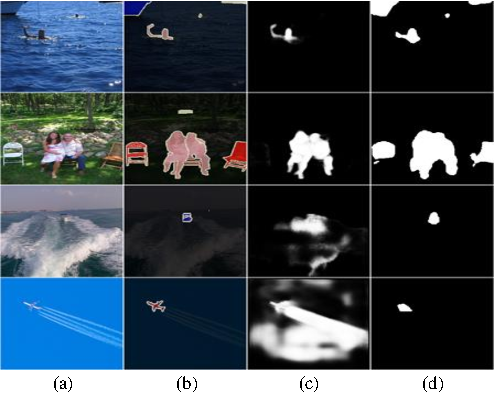
\includegraphics[width=8cm]{figures/fig_saliency_v2.pdf}
\caption{在 PASCAL VOC 2012 上估計的顯著性圖的質性範例。(a) 輸入圖像,(b) 真實值,(c) 來自 \cite{zhao2019pyramid} 的顯著性圖和 (d) 我們估計的顯著性圖。} \vspace{-2mm}
\label{fig:sal}
\end{figure}

最后,EPS 的目标函数由两部分组成:通过显著性图的{显著性损失} $
\mathcal{L}_{sal}$(在图~\ref{fig:framework} 中用红色框/箭头标记)和通过图像级标签的{多标签分类损失} $
\mathcal{L}_{cls}$(在图~\ref{fig:framework} 中用蓝色框/箭头标记)。通过联合训练这两个目标,我们可以将定位图和显著性图与互补信息协同起来——我们观察到,通过我们的联合训练策略,彼此的噪声和缺失信息得到了补充,如图~\ref{fig:sal} 所示。例如,从现成模型~\cite{hou2017deeply,nguyen2019deepusps,zhao2019pyramid} 获得的原始显著性图存在缺失和噪声信息。另一方面,我们的结果成功恢复了缺失的对象(例如,船或椅子)并去除了噪声(例如,水泡或尾迹),这显然比原始显著性图更好。因此,EPS 可以捕捉到更准确的对象边界,并将共现像素与目标对象分离。这些优势带来了显著的性能提升;表~\ref{tab:seg_quan_voc_resnet101} 报告称,EPS 在分割准确性方面显著优于现有模型,提升幅度高达 3.8--10.6%。

\subsection{显式伪像素监督}\label{section3.2}

我们解释了如何利用显著性图进行伪像素监督。显著性图的关键优势在于提供对象轮廓,可以更好地揭示对象边界。为了利用这一特性,我们将显著性图与两种情况进行匹配:前景和背景。为了使类级定位图与显著性图具有可比性,我们合并目标标签的定位图并生成前景图,$
\mathbf{M}_{fg} \in \mathbb{R}^{H \times W}$。我们还可以通过对背景图进行反转来表示前景图,背景图是背景标签的定位图 $
\mathbf{M}_{bg} \in \mathbb{R}^{H \times W}$。(稍后,我们将解释如何细化前景图以解决噪声显著性图的问题。)

具体来说,我们使用 $
\mathbf{M}_{fg}$ 和 $
\mathbf{M}_{bg}$ 估计显著性图 $
\mathbf{\hat{M}}_{s}$,如下所示:\vspace{-1mm}
\begin{equation}
\label{eq_esimate_sal}
{\small
\begin{split}
\mathbf{\hat{M}}_{s} = \lambda\mathbf{M}_{fg} + (1-\lambda)(1-\mathbf{M}_{bg}),
\end{split}}\vspace{-1mm}
\end{equation}
\noindent 其中 $\lambda \in [0, 1]$ 是一个超参数,用于调整前景图和背景图反转的加权和。(在我们的实验中,默认将 $\lambda$ 设置为 0.5,关于 $\lambda$ 的附加消融研究见补充材料。)然后,我们将显著性损失 $\mathcal{L}_{sal}$ 定义为我们估计的显著性图与实际显著性图之间的像素级差异之和。($\mathcal{L}_{sal}$ 的正式定义在第~\ref{section3.3} 节中给出。)

值得注意的是,使用预训练模型被视为弱监督学习,因此利用显著性图已被广泛接受为 WSSS 中的常见做法。尽管其受欢迎程度很高,但采用完全监督的显著性检测模型可能存在争议,因为它们使用来自不同数据集的像素级注释。在本文中,我们研究了不同显著性检测方法的效果;1)无监督和 2)完全监督的显著性检测模型(见第~\ref{section5.3} 节),并通过实验证明我们的方法使用其中任何一种都优于所有其他方法~\cite{fan2020learning,jiang2019integral,wang2018weakly, wei2016stc,yao2020saliency} 使用完全监督的显著性模型。虽然现有方法在充分利用显著性图方面有限,但我们的方法将显著性图作为伪像素监督,并将其作为边界和共现像素的线索加以利用。\vspace{1mm}
\noindent\textbf{处理显著性偏差的地图选择。} 之前,我们假设前景图可以是目标标签的定位图的并集;背景图可以是背景标签的定位图。然而,这种简单的选择规则可能与现成模型计算的显著图不兼容。例如,来自\cite{zhao2019pyramid}的显著图通常会忽略一些物体作为显著物体(例如,图~\ref{fig:concept}中火车旁的小人物)。这种系统性错误是不可避免的,因为显著性模型学习了不同数据集的统计信息。除非考虑到这种错误,否则相同的错误可能会传播到我们的模型中并导致性能下降。

为了应对系统性错误,我们开发了一种有效的策略,使用定位图和显著图之间的重叠率。具体来说,如果第 $i$ 个定位图 $\mathbf{M}_{i}$ 与显著图的重叠率超过 $\tau$\%,则将其分配给前景,否则分配给背景。形式上,前景和背景图的计算如下:\vspace{-1mm}
\begin{equation}
\label{eq_map_selection}
{\small
\begin{split}
&\mathbf{M}_{fg} = \sum_{i=1}^{C} {y_{i} \cdot \mathbf{M}_{i} \cdot \mathbbm{1}[\mathcal{O}(\mathbf{M}_i, \mathbf{M}_{s}) > \tau]}, \\
&\mathbf{M}_{bg} = \sum_{i=1}^{C} {y_{i} \cdot \mathbf{M}_{i} \cdot \mathbbm{1}[\mathcal{O}(\mathbf{M}_i, \mathbf{M}_{s}) \le \tau]} + \mathbf{M}_{C+1},
\end{split}}\vspace{-1mm}
\end{equation}
\noindent 其中 $y \in \mathbb{R}^C$ 是二进制图像级标签,$\mathcal{O}(\mathbf{M}_i, \mathbf{M}_{s})$ 是计算 $\mathbf{M}_i$ 和 $\mathbf{M}_{s}$ 之间重叠率的函数。为此,我们首先将定位图和显著图二值化:对于像素 p,$\mathbf{B}_{k}(p) = 1$ 如果 $\mathbf{M}_{k}(p) > 0.5$;否则 $\mathbf{B}_{k}(p) = 0$。$\mathbf{B}_{i}$ 和 $\mathbf{B}_{s}$ 分别是对应于 $\mathbf{M}_i$ 和 $\mathbf{M}_{s}$ 的二值化图。然后我们计算 $\mathbf{M}_i$ 和 $\mathbf{M}_{s}$ 之间的重叠率,即 $\mathcal{O}(\mathbf{M}_i ,\mathbf{M}_{s}) = |\mathbf{B}_i \cap \mathbf{B}_{s}| / |\mathbf{B}_{i}|$。我们将 $\tau=0.4$ 设置为不考虑数据集和骨干模型。在补充材料中,我们展示了我们的方法对 $\tau$ 的选择具有鲁棒性(即,$\tau$ 在 [0.3, 0.5] 范围内表现出相当的性能)。

我们将背景标签的单一定位图与未选择为前景的定位图结合起来,而不是单一的背景标签定位图。尽管简单,但我们可以绕过显著图的错误,并有效地训练显著图中被忽略的一些物体。(在表~\ref{tab:strategy}中,我们报告了所提出策略克服显著图错误的有效性。)

\subsection{联合训练过程}\label{section3.3}

使用显著图和图像级标签,EPS 的整体训练目标由两个部分组成,显著性损失 $\mathcal{L}_{sal}$ 和分类损失 $\mathcal{L}_{cls}$。首先,显著性损失 $\mathcal{L}_{sal}$ 通过测量实际显著图 $\mathbf{M}_{s}$ 和估计显著图 $\mathbf{\hat{M}}_{s}$ 之间的平均像素级距离来制定。\vspace{-1mm}
\begin{equation}
{\small
\label{loss_sal}
\mathcal{L}_{sal} = \frac{1}{H\cdot W}||\mathbf{M}_{s}-\mathbf{\hat{M}}_{s}||^{2},
}\vspace{-1mm}
\end{equation}
\noindent 其中 $\mathbf{M}_{s}$ 是从现成的显著性检测模型——PFAN~\cite{zhao2019pyramid} 训练于 DUTS 数据集~\cite{wang2017learning} 中获得的。请注意,我们的方法始终优于所有先前的艺术,无论显著性检测模型如何。

接下来,分类损失通过图像级标签 $y$ 和其预测 $\hat{y} \in \mathbb{R}^C$ 之间的多标签软边缘损失来计算,后者是对每个目标类的定位图进行全局平均池化的结果。\vspace{-1mm}
\begin{equation}
{\small
\begin{split}
\label{loss_cls}
\mathcal{L}_{cls}= - \frac{1}{C} \sum_{i=1}^{C} y_i \log{\sigma(\hat{y_i})} + (1-y_i) \log{(1 - \sigma(\hat{y_i}))},
\end{split}}\vspace{-1mm}
\end{equation}
\noindent 其中 $\sigma(\cdot)$ 是 sigmoid 函数。最后,总训练损失是多标签分类损失和显著性损失的总和,即 $\mathcal{L}_{total} = \mathcal{L}_{cls} + \mathcal{L}_{sal}$。
如图~\ref{fig:framework}所示,$\mathcal{L}_{sal}$ 涉及更新 $C+1$ 类的参数,包括目标对象和背景。同时,$\mathcal{L}_{cls}$ 仅评估 $C$ 类的标签预测,不包括背景类——来自 $\mathcal{L}_{cls}$ 的梯度不会流入背景类。然而,背景类的预测可以被 $\mathcal{L}_{cls}$ 隐式影响,因为它监督分类器的训练。

\section{实验设置}
\noindent
\textbf{数据集}。我们在两个流行的基准数据集上进行实证研究,PASCAL VOC 2012~\cite{everingham2015pascal} 和 MS COCO 2014~\cite{lin2014microsoft}。PASCAL VOC 2012 包含 21 个类(即 20 个对象和背景),分别有 1,464、1,449 和 1,456 张用于训练、验证和测试集的图像。按照语义分割的常见做法,我们使用包含 10,582 张图像的增强训练集~\cite{hariharan2011semantic}。接下来,COCO 2014 包含 81 个类,包括一个背景,分别有 82,081 和 40,137 张用于训练和验证的图像,其中不包含目标类的图像被排除,如~\cite{choe2020attention}所做。由于某些对象的真实分割标签相互重叠,我们采用 COCO-Stuff~\cite{caesar2018coco} 的真实分割标签,解决了同一 COCO 数据集上的重叠问题。

\vspace{0.5mm}
\noindent
\textbf{评估协议}。我们在 PASCAL VOC 2012 的验证集和测试集以及 COCO 2014 的验证集上验证我们的方法。PASCAL VOC 2012 测试集的评估结果来自官方 PASCAL VOC 评估服务器。此外,我们采用平均交并比(mIoU)来衡量分割模型的准确性。

\vspace{0.5mm}
\noindent
\textbf{实现细节}。我们选择 ResNet38~\cite{wu2019wider} 作为我们方法的主干网络,输出步幅为 8。所有主干模型均在 ImageNet~\cite{deng2009imagenet} 上进行预训练。我们使用批量大小为 8 的 SGD 优化器。我们的方法训练到 20k 次迭代,学习率为 0.01(最后一个卷积层为 0.1)。对于数据增强,我们使用随机缩放、随机翻转和随机裁剪到 $448 \times 448$。对于分割网络,我们采用 DeepLab-LargeFOV (V1)~\cite{chen2014semantic} 和 DeepLab-ASPP (V2)~\cite{chen2017deeplab},以及 VGG16 和 ResNet101 作为其主干网络。具体来说,我们使用四个分割网络:基于 VGG16 的 DeepLab-V1 和 DeepLab-V2,基于 ResNet101 的 DeepLab-V1 和 DeepLab-V2。更详细的设置在补充材料中。

\section{实验结果}

\subsection{处理边界和共现问题}\label{section:5.1}

\noindent\textbf{边界不匹配问题}。为了验证伪掩码的边界,我们与最先进的方法~\cite{chen2020boundary, wang2020self, zhou2016learning}比较边界的质量。我们利用 SBD~\cite{hariharan2011semantic},它提供了边界注释和 PASCAL VOC 2011 的边界基准。如~\cite{chen2020boundary}所做,边界的质量通过计算伪掩码的拉普拉斯边缘检测器的边缘以类无关的方式进行评估。然后,通过测量召回率、精确率和 F1 分数,比较预测和真实边界来评估边界质量。表~\ref{tab:boundary} 报告了我们的方法在所有三个指标上大大优于其他方法。图~\ref{fig:ablation} 中的定性示例显示,我们的方法可以比所有其他方法捕捉到更准确的边界。

\begin{figure}[t]
\centering
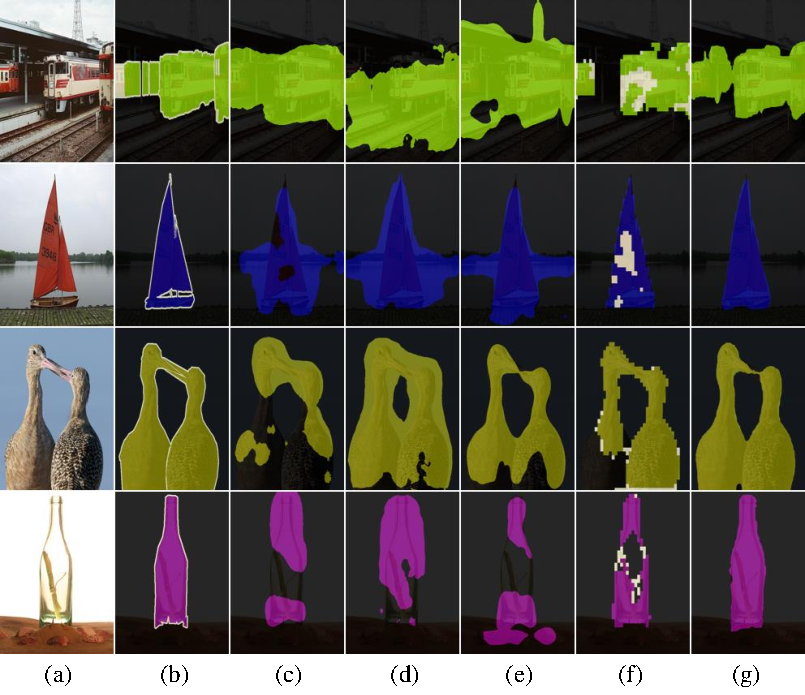
\includegraphics[width=8cm]{figures/fig_ablation.pdf}
\caption{Qualitative comparison for pseudo-masks on PASCAL VOC 2012. (a) Input images, (b) groundtruth, (c) CAM, (d) SEAM, (e) ICD, (f) SGAN and (g) our EPS.}
\label{fig:ablation} \vspace{-3mm}
\end{figure}


\begin{table}[]
\centering
{\small
\begin{tabular}{@{}lccc@{}}
\toprule
\multicolumn{1}{c}{方法}                      & 召回率(\%) & 精确率(\%) & F1-分数(\%) \\ \midrule
\multicolumn{1}{l}{CAM~\cite{zhou2016learning}\textsubscript{CVPR'16}} & 22.3        & 35.8           & 27.5           \\
\multicolumn{1}{l}{SEAM~\cite{wang2020self}\textsubscript{CVPR'20}}    & 40.2        & 45.0           & 42.5           \\
\multicolumn{1}{l}{BES~\cite{chen2020boundary}\textsubscript{ECCV'20}} & 45.5        & 46.4           & 45.9           \\
\multicolumn{1}{l}{我们的 EPS}                        & 60.0        & 73.1          & 65.9           \\ \bottomrule
\end{tabular}
}
\vspace{2mm}
\caption{在 SBD trainval 集上评估的边界准确性。请注意,BES 的结果是从~\cite{chen2020boundary}中提出的边界预测网络测量的。} \vspace{-2mm}
\label{tab:boundary}
\end{table}


\vspace{1mm}
\noindent \textbf{共现问题}。如几项研究中讨论的~\cite{huang2018weakly, kolesnikov2016seed, li2018tell, oh2017exploiting},我们观察到在 PASCAL VOC 2012 中,一些背景类经常与目标对象一起出现。我们通过使用 PASCAL-CONTEXT 数据集~\cite{mottaghi2014role} 进行定量分析,该数据集为整个场景提供像素级注释(例如,~\emph{水} 和 ~\emph{铁路})。我们选择了三个共现对;\emph{船} 和 \emph{水},\emph{火车} 和 \emph{铁路},以及 \emph{火车} 和 \emph{平台}。我们比较目标类的 IoU 和目标类与其共现类之间的 \emph{混淆率}。混淆率衡量共现类被错误预测为目标类的程度。混淆率 $m_{k,c}$ 通过 $m_{k,c} = FP_{k,c}/TP_{c}$ 计算,其中 ${FP_{k,c}}$ 是共现类 $k$ 被错误分类为目标类 $c$ 的像素数,$TP_{c}$ 是目标类 $c$ 的真阳性像素数。关于共现问题的更详细分析在补充材料中。
表~\ref{tab:co_quantitative_v4} 报告了 EPS 的混淆率始终低于其他方法。SGAN~\cite{yao2020saliency} 的混淆率与我们的方法非常相似,但我们的方法在 IoU 方面更准确地捕捉目标类别。有趣的是,SEAM 显示出较高的混淆率,甚至比 CAM 更差。这是因为 SEAM~\cite{wang2020self} 通过应用自监督训练来学习覆盖目标对象的全部范围,这很容易被目标对象的重合像素所迷惑。同时,CAM 只捕捉目标对象中最具辨别力的区域,而不覆盖较不具辨别力的部分,例如重合类。我们也可以在图~\ref{fig:ablation} 中观察到这种现象。

% 請將以下所需的套件添加到您的文件前言:
% \usepackage{booktabs}

\newcommand{\R}{\textcolor{red}}
\newcommand{\B}{\textcolor{blue}}

\begin{table}[]
\centering
{\small
\begin{tabular}{@{}llll@{}}
\toprule
\multicolumn{1}{c}{\multirow{2}{*}{方法}} & \multicolumn{1}{c}{~\emph{船} w/}   & \multicolumn{1}{c}{~\emph{火車} w/}  & \multicolumn{1}{c}{~\emph{火車} w/}  \\
& \multicolumn{1}{c}{~\emph{水}} & \multicolumn{1}{c}{~\emph{鐵路}}          & \multicolumn{1}{c}{~\emph{平台}}  \\ \midrule
\multicolumn{1}{l}{CAM~\cite{zhou2016learning}\textsubscript{CVPR'16}}              & \B{0.74} (33.1)   & \B{0.11} (52.9)   & \multicolumn{1}{l}{\B{0.09} (49.6)}   \\
\multicolumn{1}{l}{SEAM~\cite{wang2020self}\textsubscript{CVPR'20}}                 & \B{1.13} (30.7)   & \B{0.24} (48.6)   & \multicolumn{1}{l}{\B{0.20} (45.5)}   \\
\multicolumn{1}{l}{ICD~\cite{fan2020learning}\textsubscript{CVPR'20}}               & \B{0.47} (41.4)   & \B{0.11} (56.7)   & \multicolumn{1}{l}{\B{0.09} (49.2)}   \\
\multicolumn{1}{l}{SGAN~\cite{yao2020saliency}\textsubscript{ACCESS'20}}            & \B{0.10} (42.3)   & \B{0.02} (48.8)   & \multicolumn{1}{l}{\B{0.01} (36.3)}   \\
\multicolumn{1}{l}{我們的 EPS}                                                         & \B{0.10} (55.0)   & \B{0.02} (78.1)   & \multicolumn{1}{l}{\B{0.01} (73.0)}   \\ \bottomrule
\end{tabular}
}
\vspace{2mm}
\caption{與現有代表性方法處理共現問題的比較。每個條目是 {$m_{k,c}$} 在~\B{藍色}中(越低越好),括號中的 IoU(越高越好)。} \vspace{-2mm}
\label{tab:co_quantitative_v4}

\end{table}

\begin{table}[]
%\resizebox{\columnwidth}{!}{%
\centering

{\small
\begin{tabular}{@{}ccccc@{}}
\toprule
                            & 基线  & 简单   & 预定义   & 我们的自适应 \\ \midrule
\multicolumn{1}{l}{mIoU}    &66.1       & 66.5      & 67.9          & 69.4   \\ \bottomrule
\end{tabular}
}
\vspace{2mm}
\caption{地图选择策略的效果。使用不同地图选择策略的伪掩码的准确性在 PASCAL VOC 2012 训练集上进行评估。} \vspace{-2mm}
\label{tab:strategy}
\end{table}


\subsection{地图选择策略的效果}
我们评估了我们的地图选择策略在减轻显著性图误差方面的有效性。我们将三种不同的地图选择策略与不使用地图选择模块的基线进行比较。作为简单策略,前景图是所有对象定位图的并集;背景图等于背景类的定位图(即简单策略)。接下来,我们遵循简单策略,但有以下例外。几个预定类(例如,\emph{沙发}、\emph{椅子}和\emph{餐桌})的定位图被分配到背景图(即预定义类策略)。最后,所提出的选择方法利用定位图和显著性图之间的重叠率,如第~\ref{section3.2} 节所述(即我们的自适应策略)。

\begin{figure*}[t]
\centering
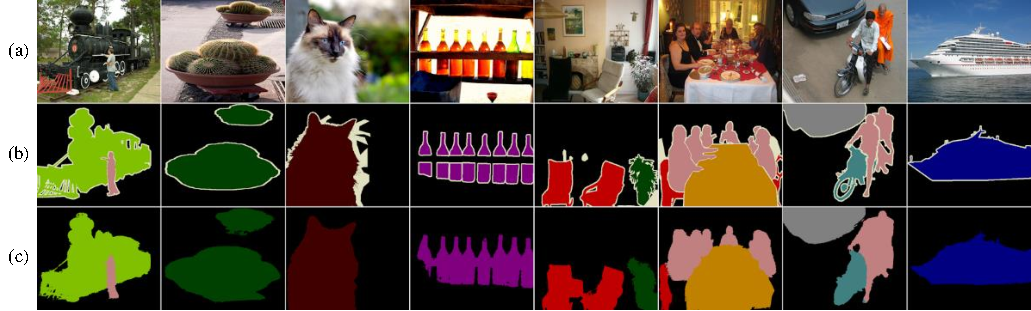
\includegraphics[width=17cm]{figures/segmentation_voc.pdf}
\caption{PASCAL VOC 2012 上分割结果的定性示例。(a) 输入图像,(b) 真实值和 (c) 我们的 EPS。}\vspace{-2mm}
\label{fig:seg_qual_voc}
\end{figure*}

\begin{table}[]
\centering
{\small
\begin{tabular}{@{}lccc@{}}
\toprule
\multicolumn{1}{c}{\multirow{2}{*}{Method}}         & w/o           & w/ &                                  w/ \\
                                                    & refinement    & CRF~\cite{krahenbuhl2011efficient}    & AffinityNet~\cite{ahn2018learning}    \\ \midrule
\multicolumn{1}{l}{CAM~\cite{zhou2016learning}\textsubscript{CVPR'16}}     & 48.0          & -                                     & 58.1                                  \\
\multicolumn{1}{l}{SEAM~\cite{wang2020self}\textsubscript{CVPR'20}}        & 55.4          & 56.8                                  & 63.6                                  \\
\multicolumn{1}{l}{ICD~\cite{chen2020boundary}\textsubscript{CVPR'20}*}     & 59.9          & 62.2                                  & -                                     \\
\multicolumn{1}{l}{SGAN~\cite{yao2020saliency}\textsubscript{ACCESS'20}*}     & 62.8          & -                                     & -                                     \\
\multicolumn{1}{l}{Our EPS}                            & 69.4          & 71.4                                  & 71.6                                  \\ \bottomrule
\end{tabular}
}
\vspace{2mm}
\caption{PASCAL VOC 2012のトレインセットで評価された擬似マスクの精度(mIoU)。*は低信頼度のピクセルが無視されることを示します。他の方法はすべてのピクセルを評価に使用します。} \vspace{-3mm}
\label{tab:refinement}
\end{table}


表~\ref{tab:strategy} 显示了我们的自适应策略可以有效处理显著性图的系统偏差。简单策略意味着在从定位图生成估计显著性图时没有考虑偏差。在这种情况下,伪掩码的性能下降,尤其是在\emph{沙发}、\emph{椅子}或\emph{餐桌}类上。使用预定义类的性能表明,通过忽略显著性图中缺失的类可以减轻偏差。然而,由于需要人工观察者进行手动选择,因此不太实用,无法为每张图像做出最佳决策。同时,我们的自适应策略可以自动处理偏差,并为给定的显著性图做出更有效的决策。

\subsection{与最先进方法的比较}
\label{section5.3}

\noindent \textbf{伪掩码的准确性。} 我们通过聚合不同尺度图像的预测结果采用多尺度推理,这是一种常用的实践,利用于~\cite{ahn2018learning,wang2020self}。然后,我们通过将我们的 EPS 与基线 CAM~\cite{zhou2016learning} 和三种最先进的方法进行比较来评估训练集中的伪掩码的准确性,即 SEAM~\cite{wang2020self}、ICD~\cite{fan2020learning} 和 SGAN~\cite{yao2020saliency}。在这里,测量训练集中伪掩码的准确性是 WSSS 中的常见协议,因为训练集的伪掩码用于监督分割模型。表~\ref{tab:refinement} 总结了伪掩码的准确性,并表明我们的方法明显优于所有现有方法,差距为 7--21\%。图~\ref{fig:ablation} 可视化了伪掩码的定性示例,确认我们的方法显著改善了对象边界,并在伪掩码质量方面显著优于三种最先进的方法。我们的方法可以捕捉对象的精确边界(第二行),因此自然覆盖对象的全部范围(第三行),并减轻重合像素(第一行)。更多示例和失败案例在补充材料中提供。

\begin{table}[]
\normalsize
\centering
{\small
\begin{tabular}{@{}lccll@{}}
\toprule
\multicolumn{1}{c}{방법}                                                              & 세그.      & 지원.  & \multicolumn{1}{c}{val} & \multicolumn{1}{c}{test} \\ \midrule
\multicolumn{1}{l}{SEC~\cite{kolesnikov2016seed}\textsubscript{ECCV'16}}                & V1        & I.    & 50.7                    & 51.7                     \\
\multicolumn{1}{l}{AffinityNet~\cite{ahn2018learning}\textsubscript{CVPR'18}}           & V1        & I.    & 58.4                    & 60.5                     \\
\multicolumn{1}{l}{ICD~\cite{fan2020learning}\textsubscript{CVPR'20}}                   & V1        & I.    & 61.2                    & 60.9                     \\
\multicolumn{1}{l}{BES~\cite{chen2020boundary}\textsubscript{ECCV'20}}                  & V1        & I.    & 60.1                    & 61.1                     \\
\multicolumn{1}{l}{GAIN~\cite{li2018tell}\textsubscript{CVPR'18}}                       & V1        & I.+S. & 55.3                    & 56.8                     \\
\multicolumn{1}{l}{MCOF~\cite{wang2018weakly}\textsubscript{CVPR'18}}                   & V1        & I.+S. & 56.2                    & 57.6                     \\
\multicolumn{1}{l}{SSNet~\cite{zeng2019joint}\textsubscript{ICCV'19}}                   & V1        & I.+S. & 57.1                    & 58.6                     \\
\multicolumn{1}{l}{DSRG~\cite{huang2018weakly}\textsubscript{CVPR'18}}                  & V2        & I.+S. & 59.0                    & 60.4                     \\
\multicolumn{1}{l}{SeeNet~\cite{hou2018self}\textsubscript{NeurIPS'18}}                 & V1        & I.+S. & 61.1                    & 60.7                     \\
\multicolumn{1}{l}{MDC~\cite{wei2018revisiting}\textsubscript{CVPR'18}}                 & V1        & I.+S. & 60.4                    & 60.8                     \\
\multicolumn{1}{l}{FickleNet~\cite{lee2019ficklenet}\textsubscript{CVPR'18}}            & V2        & I.+S. & 61.2                    & 61.9                     \\
\multicolumn{1}{l}{OAA~\cite{jiang2019integral}\textsubscript{ICCV'19}}                 & V1        & I.+S. & 63.1                    & 62.8                     \\
\multicolumn{1}{l}{ICD~\cite{fan2020learning}\textsubscript{CVPR'20}}                   & V1        & I.+S. & 64.0                    & 63.9                     \\
\multicolumn{1}{l}{Multi-Est.~\cite{fan2020employing}\textsubscript{ECCV'20}}           & V1        & I.+S. & 64.6                    & 64.2                     \\
\multicolumn{1}{l}{Split. \& Merge.~\cite{zhang2020splitting}\textsubscript{ECCV'20}}   & V2        & I.+S. & 63.7                    & 64.5                     \\
\multicolumn{1}{l}{SGAN~\cite{yao2020saliency}\textsubscript{ACCESS'20}}                & V2        & I.+S. & 64.2                    & 65.0                     \\ \midrule
\multicolumn{1}{l}{\multirow{2}{*}{우리의 EPS}}                                            & V1        & I.+S. & 66.6                    & \textbf{67.9}            \\
\multicolumn{1}{l}{}                                                                    & V2        & I.+S. & \textbf{67.0}           & 67.3                     \\ \bottomrule

\end{tabular}
}
\vspace{2mm}
\caption{PASCAL VOC 2012에서의 세그멘테이션 결과 (mIoU). 모든 결과는 VGG16을 기반으로 합니다. 모든 실험에서 최고의 점수는 굵게 표시되어 있습니다.}\vspace{-3mm}
\label{tab:seg_quan_voc_vgg16}
\end{table}

\begin{table}[]
\normalsize
\centering
{\small
\begin{tabular}{@{}lccll@{}}
\toprule
\multicolumn{1}{c}{Method}                                                              & Seg.      & Sup.  & \multicolumn{1}{c}{val} & \multicolumn{1}{c}{test} \\ \midrule
\multicolumn{1}{l}{ICD~\cite{fan2020learning}\textsubscript{CVPR'20}}                   & V1        & I.    & 64.1                    & 64.3                     \\ 
\multicolumn{1}{l}{SC-CAM~\cite{chang2020weakly}\textsubscript{CVPR'20}}                & V1        & I.    & 66.1                    & 65.9                     \\
\multicolumn{1}{l}{BES~\cite{chen2020boundary}\textsubscript{ECCV'20}}                  & V2        & I.    & 65.7                    & 66.6                     \\
\multicolumn{1}{l}{LIID~\cite{liu2020leveraging}\textsubscript{TPAMI'20}}                  & V2        & I.    & 66.5                    & 67.5                     \\
\multicolumn{1}{l}{MCOF~\cite{wang2018weakly}\textsubscript{CVPR'18}}                   & V1        & I.+S. & 60.3                    & 61.2                     \\
\multicolumn{1}{l}{SeeNet~\cite{hou2018self}\textsubscript{NeurIPS'18}}                 & V1        & I.+S. & 63.1                    & 62.8                     \\
\multicolumn{1}{l}{DSRG~\cite{huang2018weakly}\textsubscript{CVPR'18}}                  & V2        & I.+S. & 61.4                    & 63.2                     \\
\multicolumn{1}{l}{FickleNet~\cite{lee2019ficklenet}\textsubscript{CVPR'18}}            & V2        & I.+S. & 64.9                    & 65.3                     \\
\multicolumn{1}{l}{OAA~\cite{jiang2019integral}\textsubscript{ICCV'19}}                 & V1        & I.+S. & 65.2                    & 66.4                     \\
\multicolumn{1}{l}{Multi-Est.~\cite{fan2020employing}\textsubscript{ECCV'19}}           & V1        & I.+S. & 67.2                    & 66.7                     \\
\multicolumn{1}{l}{MCIS~\cite{sun2020mining}\textsubscript{ECCV'20}}                    & V1        & I.+S. & 66.2                    & 66.9                     \\
\multicolumn{1}{l}{SGAN~\cite{yao2020saliency}\textsubscript{ACCESS'20}}                & V2        & I.+S. & 67.1                    & 67.2                     \\
\multicolumn{1}{l}{ICD~\cite{fan2020learning}\textsubscript{CVPR'20}}                   & V1        & I.+S. & 67.8                    & 68.0                     \\ \midrule
\multicolumn{1}{l}{\multirow{2}{*}{Our EPS}}                                            & V1        & I.+S. & \textbf{71.0}           & \textbf{71.8}            \\
\multicolumn{1}{l}{}                                                                    & V2        & I.+S. & 70.9                    & 70.8                     \\ \bottomrule
\end{tabular}
}
\vspace{2mm}
\caption{PASCAL VOC 2012에서의 세그멘테이션 결과 (mIoU). 모든 결과는 ResNet101을 기반으로 합니다.}\vspace{-2mm}
\label{tab:seg_quan_voc_resnet101}
\end{table}

\begin{figure*}[t]
\centering
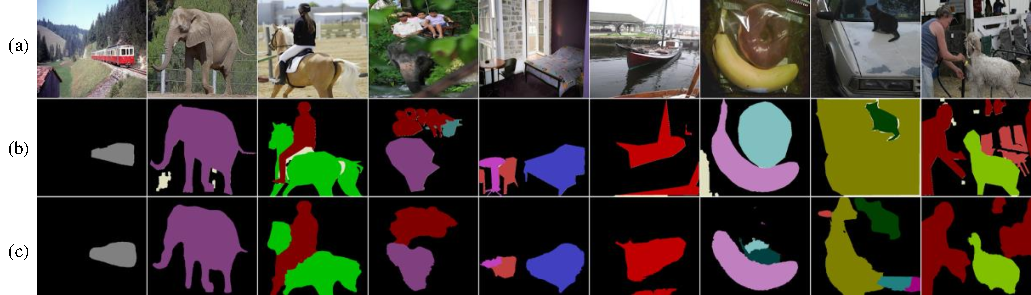
\includegraphics[width=17cm]{figures/segmentation_coco.pdf}
\caption{MS COCO 2014에서의 세분화 결과에 대한 정성적 예시입니다. (a) 입력 이미지, (b) 정답 및 (c) 우리의 EPS.}\vspace{-2mm}
\label{fig:seg_qual_coco} 
\end{figure*}


\vspace{1mm}
\noindent \textbf{分割图的准确性}。以前的方法~\cite{ahn2018learning, fan2020learning, wang2020self} 生成伪掩码并使用 CRF 后处理算法~\cite{krahenbuhl2011efficient} 或亲和网络~\cite{ahn2018learning} 对其进行细化。同时,如表~\ref{tab:refinement} 所示,我们生成的伪掩码足够准确,因此我们在没有任何额外细化的情况下训练分割网络。我们在 Pascal VOC 2012 数据集的四个分割网络上广泛评估并精确比较我们的方法与其他方法。

% Please add the following required packages to your document preamble:
% \usepackage{booktabs}
\begin{table}[]
\centering
{\small
\begin{tabular}{@{}lccc@{}}
\toprule
\multicolumn{1}{c}{Method}                                                  &Seg.       &Sup.   & \multicolumn{1}{c}{val}           \\ \midrule
\multicolumn{1}{l}{SEC~\cite{kolesnikov2016seed}\textsubscript{ECCV'16}}    & V1        &I.     & \multicolumn{1}{c}{22.4}          \\
\multicolumn{1}{l}{DSRG~\cite{huang2018weakly}\textsubscript{CVPR'18}}      & V2        &I.+S.  & \multicolumn{1}{c}{26.0}          \\
\multicolumn{1}{l}{ADL~\cite{choe2020attention}\textsubscript{TPAMI'20}}    & V1        &I.+S.  & \multicolumn{1}{c}{30.8}          \\
\multicolumn{1}{l}{SGAN~\cite{yao2020saliency}\textsubscript{ACESS'20}}     & V2        &I.+S.  & \multicolumn{1}{c}{33.6}          \\ \midrule
\multicolumn{1}{l}{Our EPS}                                                 & V2        &I.+S.  & \multicolumn{1}{c}{\textbf{35.7}} \\ \bottomrule
\end{tabular}
}
\vspace{2mm}
\caption{Segmentation results (mIoU) on MS COCO 2014. All results are based on VGG16.}\vspace{-2mm}
\label{tab:seg_quantitative_coco}
\end{table}

我们的方法在分割网络方面表现显著优于其他方法。表~\ref{tab:seg_quan_voc_vgg16} 报告了在相同的 VGG16 主干网络下,我们的方法比其他方法更准确。此外,我们在 VGG16 上的结果与基于更强大主干网络(\ie 表~\ref{tab:seg_quan_voc_resnet101} 中的 ResNet101)的其他现有方法相当甚至更优。我们的方法也显示出相对于现有方法的明显改进。最后,表~\ref{tab:seg_quan_voc_resnet101} 显示,我们的方法(在基于 ResNet101 的 DeepLab-V1 和显著性图下)在 PASCAL VOC 2012 数据集上达到了新的最先进性能(验证集为 71.0,测试集为 71.8)。我们强调,现有最先进模型的增益约为 1\%,而我们的方法比之前的最佳记录高出 3\% 以上。图~\ref{fig:seg_qual_voc} 可视化了我们在 PASCAL VOC 2012 上的分割结果的定性示例。这些结果证实了我们的方法提供了准确的边界,并成功解决了共现问题。

在表~\ref{tab:seg_quantitative_coco} 中,我们进一步在 COCO 2014 数据集上评估了我们的方法。我们使用基于 VGG16 的 DeepLab-V2 作为分割网络,与 COCO 数据集中的最先进 WSSS 模型 SGAN~\cite{yao2020saliency} 进行比较。我们的方法在验证集上达到了 35.7 mIoU,比 SGAN~\cite{yao2020saliency} 高出 1.9\%。因此,我们在 COCO 2014 数据集上达到了新的最先进准确性。在这两个数据集上超越现有最先进方法的出色表现证实了我们方法的有效性;通过充分利用定位图和显著性图,它成功地正确捕捉了目标对象的整体,并弥补了现有模型的不足。图~\ref{fig:seg_qual_coco} 显示了 COCO 2014 数据集上的分割结果的定性示例。当少数对象出现且没有遮挡时,我们的方法表现良好,但在处理许多小对象时效果较差。我们的方法的更多示例和失败案例在补充材料中提供。

\vspace{1mm}
\noindent \textbf{显著性检测模型的效果}。为了研究不同显著性检测模型的效果,我们采用了三种显著性模型;PFAN~\cite{zhao2019pyramid}(我们的默认模型),DSS~\cite{hou2017deeply} 被 OAA~\cite{jiang2019integral} 和 ICD~\cite{fan2020learning} 使用,以及 USPS~\cite{nguyen2019deepusps}(\ie,无监督检测模型)。在基于 Resnet101 的 DeepLab-V1 下的分割结果(mIoU)分别为 71.0/71.8(PFAN),70.0/70.1(DSS),和 68.8/69.9(USPS)(验证集和测试集)。这些分数支持我们的 EPS 使用任何三种不同的显著性模型仍然比表~\ref{tab:seg_quan_voc_resnet101} 中的所有其他方法更准确。值得注意的是,我们的 EPS 使用无监督显著性模型优于所有使用监督显著性模型的现有方法。

\section{结论}
我们提出了一种新颖的弱监督分割框架,即 \emph{显式伪像素监督(EPS)}。受定位图和显著性图之间互补关系的启发,我们的 EPS 从结合显著性图和定位图的伪像素反馈中学习。由于我们的联合训练方案,我们成功地补充了两侧的噪声或缺失信息。因此,我们的 EPS 能够捕捉精确的对象边界,并丢弃非目标对象的共现像素,显著提高了伪掩码的质量。广泛的评估和各种案例研究证明了我们 EPS 的有效性和出色的表现,以及在 PASCAL VOC 2012 和 MS COCO 2014 数据集上 WSSS 的新最先进准确性。

\noindent\textbf{致谢。}
我们感谢 Duhyeon Bang 和 Junsuk Choe 的反馈。该研究得到了韩国 NRF 基础科学研究计划的支持,由 MSIP 资助(NRF-2019R1A2C2006123, 2020R1A4A1016619),由 MSIT 资助的 IITP 资助(2020-0-01361,人工智能研究生院计划(延世大学)),以及由韩国政府资助的韩国医疗设备开发基金资助(项目编号:202011D06)。

{\small
\bibliographystyle{ieee_fullname}
\bibliography{egbib}
}

\end{document}
